\section{Statistical Analysis, Pipeline Automation, and System Launcher}

\subsection{Purpose and Design}
The analysis and automation subsystem encompasses the modules responsible for data analytics, batch pipeline orchestration, and system initialization: the statistical analysis engine (\texttt{src/analyzer.py}), the sequential pipeline runner (\texttt{bin/run\_pipeline.sh}), and the master system launcher (\texttt{./sysmon}).

\textbf{1. Statistical Analysis Engine (\texttt{src/analyzer.py}):}
The analyzer transforms cleaned high-frequency telemetry into statistical summaries, predictive capacity forecasts, and anomaly indicators. 
\begin{itemize}
    \item \textbf{Input Data and Fields:} Ingests \path{data/clean/metrics.csv} (19 fields: 16 raw metrics plus \texttt{is\_filled}, \texttt{is\_gap}, \texttt{is\_outlier}), process records from \path{data/raw/processes_YYYYMMDD.csv} (6 fields: \texttt{epoch}, \texttt{pid}, \texttt{command}, \texttt{cpu\_pct}, \texttt{mem\_pct}, \texttt{rank}), and system metadata from \path{data/system_info.json}.
    \item \textbf{Rolling Multi-Window Metrics:} Computes five core statistical metrics (mean, minimum, maximum, 95th percentile, and standard deviation) across four sliding windows (\texttt{1h}, \texttt{24h}, \texttt{7d}, \texttt{all}).
    \item \textbf{Hourly Averages:} Bins timestamps into 24 daily hours ($0\dots 23$) to uncover diurnal human and batch operational patterns. 
    \item \textbf{Core-Normalized Top Processes:} Averages command CPU and memory across sample windows and normalizes CPU by physical cores: $\text{avg\_cpu\_norm} = \min\left(100.0, \frac{\text{avg\_cpu}}{\text{cpu\_cores}}\right)$, aligning process reporting with desktop resource managers. 
\end{itemize}
Sized windows allow immediate reaction (\texttt{1h}), diurnal tracking (\texttt{24h}), and baseline trends (\texttt{7d}, \texttt{all}). Safe floating-point parsing (\texttt{parse\_float}) returns \texttt{None} on empty or non-numeric tokens without throwing exceptions, allowing non-GPU hosts to produce \texttt{null} statistics gracefully. Output is written atomically to \path{data/stats.json} via temporary file rename to prevent partial reads by the web API.

\textbf{2. Pipeline Runner (\texttt{bin/run\_pipeline.sh}):}
The pipeline runner coordinates the batch processing lifecycle. It sequentially executes Cleaner $\rightarrow$ Analyzer $\rightarrow$ Alerts. The runner enforces fail-fast error isolation: if any stage exits with a non-zero code, execution halts immediately and logs the failure to \path{data/pipeline.log}. The script atomically writes duration and status to \path{data/pipeline_status.json} using a process-isolated temporary file renamed via POSIX \texttt{mv}. To eliminate unnecessary computation, the runner implements file fingerprint caching (\texttt{.pipeline\_raw\_stamp}): if raw CSV file sizes and modification timestamps match the previous run, cleaner and analyzer stages are safely skipped. Subprocess thread explosions were eliminated by explicitly exporting \texttt{OPENBLAS\_NUM\_THREADS=1}, \texttt{OMP\_NUM\_THREADS=1}, and \texttt{MKL\_NUM\_THREADS=1}.

\textbf{3. Master System Launcher (\texttt{./sysmon}):}
The root \texttt{./sysmon} executable enables one-command startup on a fresh clone without manual terminal configuration. It detects or builds the Python virtual environment (\texttt{.venv}), verifies dependencies from \texttt{requirements.txt} (bypassing pip on subsequent runs via fast Python import checks), initializes baseline configurations (\texttt{config/sysmon.conf} and \texttt{config/thresholds.conf} via \texttt{--init-defaults}), starts the Flask server, and automatically launches the browser dashboard.

\subsection{Inputs and Outputs}
Table~\ref{tab:analysis_automation_io} summarizes the interface contracts, configurations, and outputs of the analyzer, pipeline runner, and launcher.

\begin{table}[htbp]
    \centering
    \small
    \begin{tabularx}{\textwidth}{llXX}
        \toprule
        File / Artifact & Format & Written By & Read By \\
        \midrule
        \texttt{config/sysmon.conf} & INI & Master Launcher / User & Pipeline Runner, Server \\
        \texttt{config/thresholds.conf} & INI & Master Launcher / Alerts & Alert Engine, Web API \\
        \texttt{data/clean/metrics.csv} & CSV (19 cols) & Data Cleaner & Statistical Analyzer \\
        \texttt{data/raw/processes\_*.csv} & CSV (6 cols) & Bash Collector & Statistical Analyzer \\
        \texttt{data/stats.json} & JSON & Statistical Analyzer & Flask Server (\texttt{/api/stats}) \\
        \texttt{data/pipeline\_status.json} & JSON & Pipeline Runner & Flask Server (\texttt{/api/status}) \\
        \texttt{data/.pipeline\_raw\_stamp} & Plain Text & Pipeline Runner & Pipeline Runner (Cache) \\
        \bottomrule
    \end{tabularx}
    \caption{Analysis, Pipeline, and Launcher Interface Artifacts}
    \label{tab:analysis_automation_io}
\end{table}

\subsection{Testing and Results}
The subsystem was validated with exhaustive test suites in \texttt{tests/test\_analyzer.py} and \texttt{tests/test\_pipeline.py}. The analyzer test suite verified mathematical correctness on hand-crafted 3-row inputs with known mean/std/p95, single-row edge cases, zero-variance flatlines, negative slopes, empty GPU rows, and core normalization. The pipeline tests validated fail-fast error halts, schema conformance of \texttt{pipeline\_status.json}, and launcher CLI flags (\texttt{--help}, \texttt{--init-defaults}, \texttt{--no-browser}).

\begin{figure}[htbp]
    \centering
    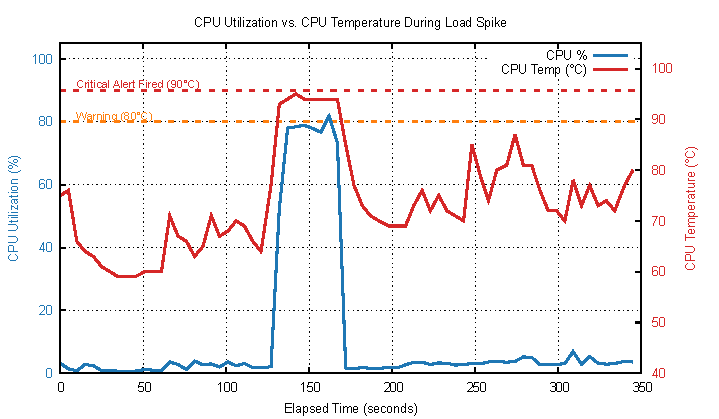
\includegraphics[width=0.88\textwidth]{figures/cpu_temp_alert.pdf}
    \caption{Real Telemetry: CPU Utilization vs. Package Temperature During Load Spike}
    \label{fig:cpu_temp_alert}
\end{figure}

The analyzer was further evaluated on real monitoring data collected over 2 days (November 12--13, 2026) across team hardware, comprising 4,778 raw rows read by the cleaner, 4,814 clean metric rows, and 23,886 process records.

Figure~\ref{fig:cpu_temp_alert} displays an empirical load event from this dataset. Under load, CPU utilization and package temperature rose synchronously; CPU jumped from 2.1\% to 78.4\%, driving temperature from 64$^\circ$C to 95$^\circ$C. The alert engine triggered \texttt{cpu\_temp\_warning} at 80$^\circ$C and \texttt{cpu\_temp\_critical} at 90$^\circ$C, automatically resolving once temperature subsided to 77$^\circ$C.

\subsection{Limitations}
The disk forecasting model assumes linear capacity consumption and cannot anticipate sudden non-linear burst writes or manual file deletions. The pipeline runner is triggered on a fixed timer rather than reactively on filesystem events.
